Strategy II}

\begin{table}
    \centering
    \begin{tabular}{clcccccc}\toprule
         &   $\alpha$ & $\beta$ & $\gamma$ & $\delta$ & $\gamma_1$ & $\gamma_2$ & $k$ \\
         \midrule
         Herring 1      & 0.1990 & -3.0000 & 0.0000 & 0.0005 &  &  &  \\
         Cod 1          &  &  &  &  & 2.2675 & 1.1415 & -0.0133 \\
         Herring 2      & 3.0000 & -0.6258 & 4.0000 & 0.0010 &  &  &  \\
         Cod 2          &  &  &  &  & 2.4354 & 2.9190 & 1.0000 \\
         Herring 3      & 0.3794 & -3.0000 & 0.9830 & 0.0010 &  &  &  \\
         Cod 3          &  &  &  &  & 3.0000 & 0.5114 & 0.1033 \\
         Herring 4      & 0.0527 & -3.0000 & 4.0000 & 0.0004 &  &  &  \\
         Cod 4          &  &  &  &  & 3.0000 & 1.0176 & 0.8409 \\
         Herring 5      & 2.4230 & -0.7872 & 3.5334 & 0.0009 &  &  &  \\
         Cod 5          &  &  &  &  & 2.5015 & 2.9897 & 0.9327 \\ \bottomrule
    \end{tabular}
    \caption{Initial results using strategy II}
    \label{tab:initial_results}
\end{table}
\begin{figure}
    \centering
    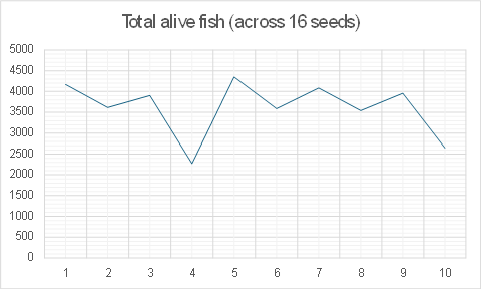
\includegraphics[width=0.75\linewidth]{fig/initial+results.png}
    \label{fig:initial_results}
    \caption{First 5 generations using strategy II, 5 predators over 10 minutes, starting at 300 fish per seed}
\end{figure}
The model was initially trained over 5 generations, using hunting strategy II. Within the five generations, there was not as much convergence as hoped as shown in \ref{fig:initial_results}, although this may change with more generations. Each generation did successfully improve the total alive herring in the relevant direction however.\par
The resultant parameters were also unexpected. All aside from $\gamma_2$ were at their maximum or minimum in at least one optimisation. It was always beneficial for herring to not align in velocity, but forming loose clusters was generally beneficial. Some parameters, particularly $\alpha, \beta$ and $\gamma_2$ are also highly correlated with each other.
\begin{figure}
    \centering
    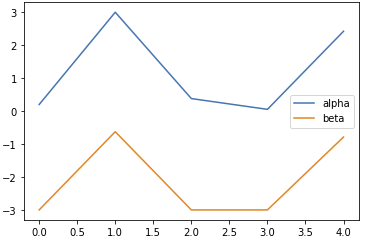
\includegraphics[width=0.75\linewidth]{fig/alpha_beta_1.png}
    \caption{Comparison of $\alpha$ and $\beta$ across generations}
    \label{fig:alpha_beta}
\end{figure}
As shown in \ref{fig:alpha_beta}, a high $\alpha$ correlates with a high $\beta$. It also correlates with predators being particularly successful on their next round, shown in generations 4 and 10 in \ref{fig:initial_results}. This suggests two different optimal options for herring that are flipped between depending on cod behaviour.\par
A more detailed commentary and visualisations of the generations can be found in Appendix A.1.
\subsection{Strategy III}
These loose schools with fish attempting to move away from the centre is not visible in nature, meaning the results from strategy II are likely unrealistic. The generation was therefore retried on strategy III.\par
Further research into herring swimming speeds also suggest that the previous estimate of a maximum speed of $0.6ms^{-1}$\cite{Giske2008_EmergingSchoolStructures} is a maximum idle velocity, and instead immature herring can reach up to $1.34ms^{-1}$, sustaining speeds of $1ms^{-1}$ for over a minute. As the simulation is of adult herring and only 10 minutes long, the maximum velocity is also modified to $1ms^{-1}$.\\
(include overview of results + brief analysis, more detail in appendix)\\
(include retry on strategy II as another subsection)\\
(include retry on more realistic strategy as another subsection, with obstacles)
\section{